% !BIB TS-program = biber
% !BIB program = biber
\documentclass[a4paper,12pt]{book}
\usepackage[utf8]{inputenc}
\usepackage{lmodern,textcomp}
\usepackage{graphicx}
\usepackage{booktabs}
\usepackage{tabularx}
\usepackage{tikz}
\usepackage{url}
\usepackage{wrapfig}


\usepackage[
backend=biber,
style=apa,
natbib=true,
sortlocale=en_US,
url=true, 
doi=true,
eprint=false
]{biblatex}
\addbibresource{references.bib}

%to make line breaks possible at more parts within \texttt
\renewcommand{\texttt}[1]{%
	\begingroup
	\ttfamily
	\begingroup\lccode`~=`/\lowercase{\endgroup\def~}{/\discretionary{}{}{}}%
	\begingroup\lccode`~=`[\lowercase{\endgroup\def~}{[\discretionary{}{}{}}%
	\begingroup\lccode`~=`.\lowercase{\endgroup\def~}{.\discretionary{}{}{}}%
	\begingroup\lccode`~=`(\lowercase{\endgroup\def~}{(\discretionary{}{}{}}%
	\catcode`/=\active\catcode`[=\active\catcode`.=\active\catcode`(=\active
	\scantokens{#1\noexpand}%
	\endgroup
}
        
\usepackage[colorinlistoftodos]{todonotes}


\usepackage{listings}
\lstset{
	basicstyle=\scriptsize\ttfamily,
	columns=flexible,
	breaklines=true,
	numbers=left,
	%stepsize=1,
	numberstyle=\tiny,
	backgroundcolor=\color[rgb]{1,0,.4}
}

\lstnewenvironment{exampler}{\lstset{basicstyle=\scriptsize\ttfamily,
		columns=flexible,
		breaklines=true,
		numbers=left,
		%stepsize=1,
		numberstyle=\tiny,
		backgroundcolor=\color[rgb]{0.3,0.3,1}}}{}

\lstnewenvironment{ex_r_out}{\lstset{basicstyle=\scriptsize\ttfamily,
		columns=flexible,
		breaklines=true, 
		numbers=left,
		%stepsize=1,
		numberstyle=\tiny,
		backgroundcolor=\color[rgb]{0.3,0.3,1}}}{}

\lstnewenvironment{ex_r_in}{\lstset{basicstyle=\scriptsize\ttfamily,
		columns=flexible,
		breaklines=true,
		numbers=left,
                showlines=true,
		%stepsize=1,
		numberstyle=\tiny,
		backgroundcolor=\color[rgb]{0.5,0.5,1}}}{}

\lstnewenvironment{ex_py_out}{\lstset{basicstyle=\scriptsize\ttfamily,
		columns=flexible,
		breaklines=true,
		numbers=left,
		%stepsize=1,
		numberstyle=\tiny,
		backgroundcolor=\color[rgb]{0,0.6,.25}}}{}

\lstnewenvironment{ex_py_in}{\lstset{basicstyle=\scriptsize\ttfamily,
		columns=flexible,
		breaklines=true,
		numbers=left,
		%stepsize=1,
                showlines=true,
		numberstyle=\tiny,
		backgroundcolor=\color[rgb]{0.2,0.6,0.5}}}{}

\lstnewenvironment{examplepy}{\lstset{basicstyle=\scriptsize\ttfamily,
		columns=flexible,
		breaklines=true,
		numbers=left,
		%stepsize=1,
		numberstyle=\tiny,
		%backgroundcolor=\color[rgb]{.7,.7,.7}}}{}
		backgroundcolor=\color[rgb]{0,.6,.25}}}{}

\newcommand{\refsec}[1]{Section~\ref{sec:#1}}
\newcommand{\reffig}[1]{Figure~\ref{fig:#1}}
\newcommand{\reftab}[1]{Table~\ref{tab:#1}}

\newcommand{\code}[1]{\texttt{#1}}

\newcommand{\note}[1]{\noindent\fbox{
  \begin{minipage}{\textwidth}
    \textbf{Note:} #1
  \end{minipage}}}


\lstnewenvironment{terminal}{\lstset{basicstyle=\scriptsize\ttfamily,
		columns=flexible,
		breaklines=true,
		numbers=left,
		%stepsize=1,
		numberstyle=\tiny,
		backgroundcolor=\color[rgb]{.7,.7,.7}}}{}



% \includeonly{chapter02/chapter02}

\begin{document}

\author{Wouter van Atteveldt, Damian Trilling, Carlos Arcila Calder\'on}
\title{Computational Analysis of Communication}
\date{\today}

\frontmatter
\maketitle
\tableofcontents

\mainmatter

\setcounter{chapter}{1}
\chapter{Getting started: Fun with data and visualizations}
\label{chap:fundata}

\begin{abstract}{Abstract}
  This chapter gives a lightning tour of some of the cool (and informative) things you can do with R and Python.
  Starting from a dataset of tweets about COVID-19, we show how you can analyze this data using
  text analysis, network analysis, and using geographic information.
  The goal of this chapter is not to teach you all these techniques in detail.
  Rather, each of the examples showcases a possibility and guides you to the chapter where it will be explained in more detail.
  So don't worry too much about understanding every line of code, but relax and enjoy the ride!
\end{abstract}

\keywords{basics of programming}

\begin{objectives}
\item Get an overview of the possibilities of R and Python for data analysis and visualization
\item Understand how different aspects of data gathering, cleaning, and analysis work together
\item Have fun with data and visualizations!
\end{objectives}

\newpage
\begin{feature}
  \textbf{Packages used in this chapter}\\
  Since this chapter showcases a wide variety of possibilities,
  it relies on quite a number of third party packages.
  If needed, you can install these packages with the code below
  (see \refsec{installing} for more details):
  \doublecodex{chapter02/chapter02install}
  \noindent After installing, you need to import (activate) the packages every session:
  \doublecodex{chapter02/chapter02library}
\end{feature}


\section{Fun with Tweets}

The goal of this chapter is to showcase how you can use R or Python to quickly and easily
run some impressive analyses of real world data.
For this purpose, we will be using a data set of tweets about the COVID pandemic that is
engulfing much of the world at the time this book is written.
Of course, tweets are probably only representative for what is said on Twitter,
but the data are (semi-)public and rich, containing text, location, and network characteristics.
This makes them ideal for exploring the many ways in which we can analyse and visualize information
with Python and R. 

\refex{funtweets} shows how you can read this data set into memory using a single command.
Note that this does not retrieve the tweets from Twitter itself, but rather downloads
our cached version of the tweets.
Below we will show how you can download tweets and location data yourself, but to make sure
we can get down to business immediately we will start from this cached version. 

\begin{ccsexample}
\codex[caption=R Code]{chapter02/tweets.r}
\codex[caption=Output]{chapter02/tweetsb.r.out}
\caption{Retrieving cached tweets about COVID}\label{ex:funtweets}
\end{ccsexample}

As you can see, the dataset contains almost ten thousand tweets, listing their
sender, their location and language, the text, the number of retweets, and whether it was a reply (retweet).
You can read the start of the three most retweeted messages, which contain one (political) tweet from India
and two seemingly political and factual tweets from the United States.

\paragraph{My first bar plot} Before diving into the textual, network, and geographic data in the data set,
let's first make a simple visualization of the date at which the tweets are posted.
\refex{funtime} does this in two steps:
First, the number of tweets per hour is counted with an aggregation command.
Next, a bar plot is made of this calculated value with some options to make it look relatively clean and professional.
If you want to play around with this, you can for example try to plot the amount of tweets per language,
or turn it into a line plot. 
For more information on visualization, please see \refchap{eda}.
See \refchap{datawrangling} for an in-depth explanation of the aggregation command. 

\pyrex[caption=Barplot of tweets over time,input=r,output=r,format=png]{chapter02/funtime}

\section{Fun with textual data}

\paragraph{Corpus Analysis} Next, we can analyse which hash tags are most frequently used in this data set.
\refex{funcloud} does this by creating a \concept{document-term matrix} using the package \pkg{quanteda} (in R)
or \sklearn (in Python).
The code shows a number of steps that are made to create the final results, each of which represent
researcher choices about which data to keep and what to discard as noise.
In this case,  we select English tweets, convert text to lower case, remove stop words, and keep only words that start with \#,
while dropping words starting with \verb+#corona+ and \verb+#covid+.
To play around with this example,
see if you can adjust the code to e.g. include all words or only at-mentions instead of the hash tags
and make a different selection of tweets, for example Spanish language tweets or only popular (retweeted) tweets.
Please see \refchap{dtm} if you want to learn more about corpus analysis,
and see \refchap{datawrangling} for more information on using \fn{filter} to make selections. 

\pyrex[caption=My First Tag Cloud,input=r,output=r,format=png]{chapter02/funcloud}

\paragraph{Topic Model}
Where a word cloud (or tag cloud) shows which words occur most frequently,
a \concept{topic model} analysis which words co-occur in the same documents.
Using the most common topic modeling algorithm, Latent Dirichlet Allocation or LDA,
\refex{funlda} explores the tweets by automatically clustering the tags selected earlier into 10 \emph{topics}.
Topic modeling is non-deterministic -- if you run it again you can get slightly different topics,
and topics are swapped around randomly as the topic numbers have no special meaning.
Thus, we set the computer's random seed to ensure that if you run it again you get the same results.
As you can see, some topics seem easily interpretable (such as topic 6 about economic consequences,
and topic 7 about masks and prevention), it is always recommended to inspect the clustered documents
and edge cases in addition to the top words (or tags) as shown here.
You can play around with this example by e.g. using a different selection of words
(modifying to code of \refex{funcloud}) or changing the number of topics.
You can also change (or remove) the random seed and see how running the same model multiple times give different results. 
Please see \refsec{lda} for more information about fitting, interpreting, and validating topic models.

\pyrex[caption=Topic Model of the COVID tags,input=r,output=r,format=table]{chapter02/funlda}

\section{Fun with Visualizing Geographic information}
For the final set of examples, we will use the location information contained in the twitter data.
This information is based on what twitter users enter into their profile, and as such it is incomplete and noisya
with many users giving a nonsensical location such as `Ethereally here' or not filling in any location at all.
However, if we assume that most users that do enter a proper location (such as Lahore or Florida in the top tweets displayed above),
we can use it to map where most tweets are coming from.

The first step in this analysis is to resolve a name such as `Lahore, Pakistan' to its geographical coordinates (in this case, about 31 degrees north and 74 degrees east). This is called geocoding, and both Google maps and Open Street Maps can be used
to perform this automatically.
As with the tweets themselves, we will use a cached version of the geocoding results here so we can proceed directly.
At the end of this chapter we will show the code that was used to create this file so you can play around with it as well. 

\refex{funmap} shows how this data can be used to create a map of twitter activity.
First, the cached user data is retrieved, showing the correct location for Lahore but also
illustrating the noisiness of the data with the location `Un peu partout'.
Next, this data is \concept[joining]{joined} to the twitter data, so the coorinates are filled in where known.
Finally, we plot this information on a map, showing tweets with more retweets as larger dots.
See \refchap{eda} for more information on visualization.

\pyrex[caption=Location of COVID tweets,input=r,output=r,format=png]{chapter02/funmap}


\paragraph{Combining textual and structured information}
Since we know the location of a subset of our tweet's users,
we can differentiate between e.g. American, European, and Asian tweets.
\refex{funcompare} creates a very rough identification of North American tweets,
and uses that to compute the relative frequency of words in those tweets compared to the rest.
Not surprisingly, those tweets are much more about American politics, locations, and institutions.
The other tweets talk about UK politics but also use a variety of names to refer to the pandemic.
To play around with this, see if you can isolate e.g. Asian or South American tweets,
or compare spanish tweets from different locations.

\pyrex[caption=Corpus comparison: North American tweets vs. the rest,input=r,output=r,format=png]{chapter02/funcompare}

\section{Fun with Networks}

Twitter, of course, is a social network as well as a microblogging service:
users are connected to other users because they follow each other and retweet and like each others' tweets.
Using the \verb+reply_to_screen_name+ column, we can inspect the retweet network contained in the COVID tweet data set.
\refex{fungraph} first uses the data summarization commands from \tidyverse\ (R) and \pandas\ (python) to
create a data frame of connections or \concept{edges} listing how often each user retweets each other user.
The second code block shows how the \pkg{igraph} package is used to convert this edge list into a graph.
From this graph, we select only the largest connected component and use a clustering algorihtm to analyse which
nodes (users) form cohesive subnetworks.
Finally, a number of options are used to set the color and size of the edges, nodes, and labels,
and the resulting network is plotted.
As you can see, the central node is Donal Trump, who is retweeted by a large number of users,
some of which are then retweeted by other users.
You can play around with different settings for the plot options,
or try to filter e.g. only tweets from a certain language. 
You could also easily compute social network metrics such as centrality on this network,
and/or export the network for further analysis in specialized social network analysis software.
See \refchap{network} for more information on network analysis,
and \refchap{datawrangling} for the summarization commands used to create the edge list.

\begin{ccsexample}
  \codex[caption=R Code]{chapter02/fungraph.r}
  \codexoutputtable{chapter02/fungraph.r}
  \codex[caption=R Code]{chapter02/fungraphb.r}
  \codexoutputpng{chapter02/fungraphb.r}
\caption{Retweet nework in the COVID tweets}\label{ex:fungraph}
\end{ccsexample}

\paragraph{Geographic networks}
In the final example of this chapter, we will combine the goegraphic and network information to
show which regions of the world interact with each other.
For this, in \refex{fungeonet} we join the user information to the edges data frame created above twice:
once for the sender, once for the replied-to user.
Then, we adapt the earlier code for plotting the map by adding a line for each node in the network.
As you can see, users in the main regions (US, EU, India) mostly interact with each other,
with almost all regions also interacting with the US.

\pyrex[caption=Reply Network of Tweets,input=r,output=r,format=png]{chapter02/fungeonet}



\chapter{Programming concepts for data analysis}
\label{chap:programmingconcepts}

\begin{abstract}{Abstract}
  This chapter introduces readers to the basics of programming, data types, control structures, and functions
  in Python and R. It
explains how to deal with objects, statements, expressions, variables
and different types of data, and shows how to create and understand
simple control structures such as loops and conditions.
\end{abstract}

\keywords{basics of programming}

\begin{objectives}
\item Understand objects and data types
\item Write control structures
\item Use functions and methods
\end{objectives}

\newpage
\begin{feature}
  \textbf{Packages used in this chapter}\\
  This chapter focuses on the built-in capabilities of Python and R,
  so it does not rely on many packages.
  For R, only \index{glue}\emph{glue} is used (which allows nice text formatting).
  For Python, we only use the packages \index{numpy}\emph{numpy} and \index{pandas}\emph{pandas}
  for data frame support.
  If needed, you can install these packages with the code below
  (see Section~\ref{sec:installing} for more details).
  \doublecodex{chapter03/chapter03install}
  \noindent After installing, you need to import (activate) the packages every session:
  \doublecodex{chapter03/chapter03libraries}
\end{feature}


\section{About Objects and Data Types}
\label{sec:datatypes}

Now that you have seen what R and Python can do in Chapter~\ref{chap:fundata},
it is time to take a small step back and learn more about how it all actually works under the hood.

In both languages, you write a
\emph{script} or \emph{program} containing the commands for the
computer.  But before we get to
some real programming and exciting data analyses, we need to understand
how data can be represented and stored.

No matter whether you use R or Python, both store your data in memory as \emph{objects}.
Each of these objects has a name, and you create them by
assigning a value to a name. For example, the command \verb|x=10|
creates a new object\footnote{In both R and Python, the equals
  sign (\verb|=|) can be used to assign values. In R, however, the
  traditional way of doing this is using an arrow (\verb|<-|). In
  this book we will use the equals sign for assignment in both
  languages, but remember that for R, \verb|x=10| and
  \verb|x<-10| are essentially the same.}, named \texttt{x}, and stores the value 10
in it.  This object is now stored in memory and can be used in later
commands. Objects can be simple values such as the number 10, but they can also
be pieces of text, whole data frames (tables), or analysis results.
We call this distinction the \emph{type} or \emph{class} of an
object. 

\begin{feature}
\textbf{Objects, pointers, and variables.} In programming, a distinction is
  often made between an object (such as the number 10) and the
  variable in which it is stored (such as \texttt{x}). The latter is also called a ``pointer''.
  However, this distinction is not very relevant for most of our
  purposes. Moreover, in statistics, the word variable often refers to a
  column of data, rather than to the name of, for instance, the object
  containing the whole data frame (or table).  For that
  reason, we will use the word \emph{object} to refer to both the
  actual object or value and its name. (If you want some extra food
  for thought and want to challenge your brain
  a bit, try to see the relationship between the idea of a pointer and
  the discussion about mutable and immutable objects below.)
\end{feature}

Let us create an object that we call \verb|a| (an arbitrary name, you can use
whatever you want), assign the value 100 to it, and use the class\index{class@\texttt{class}}
function (R) or type\index{type@\texttt{type}} function (Python) to check what kind of
object we created (Example~\ref{ex:var1}).
As you can see, R reports the type of the number as ``numeric'', while Python reports it
as ``int'', short for integer or whole number.  Although they use
different names, both languages offer very similar data types.
Table~\ref{tab:types} provides an overview of some common basic data types.

\pyrex[output=both,caption=Determining the type of an object]{chapter03/var1}

% [WvA] I don't think this command is used anywhere?
%\newcommand{\fndouble}{In R, double and numeric can generally be used
%  interchangeably (there is a subtle difference, but that is not
%  relevant here).}

\begin{table}
  \caption{\label{tab:types}Most used basic data types in Python and R}{
  \begin{tabularx}{\textwidth}{lllll}
    \toprule
    \multicolumn{2}{c}{Python} & \multicolumn{2}{c}{R}& Description \\
    \cmidrule(lr){1-2}    \cmidrule(lr){3-4}\\
    Name & Example & Name & Example \\
    \midrule
    int   & \verb+1+             & integer   & \verb+1L+             & whole numbers \\
    float & \verb+1.3+           & numeric   & \verb+1.3+           & numbers with decimals \\
    str   & \verb+"Spam", 'ham'+ & character & \verb+"Spam", 'ham'+ & textual data  \\
    bool  & \verb+True, False+   & logical   & \verb+TRUE, FALSE+   & the truth values \\
    \bottomrule
  \end{tabularx}}{}
\end{table}
    


Let us have a closer look at the code in Example~\ref{ex:var1} above.
The first line is a command to create the object \emph{a} and store
its value 100; and the second is illustrative and will give you the
class of the created object, in this case ``numeric''. Notice that we
are using two native functions of R, \index{print}\texttt{print} and \index{class}\texttt{class}, and
including \verb|a| as an argument of \index{class}\texttt{class}, and the very same
\index{class(a)}\texttt{class(a)} as an argument of \index{print}\texttt{print}. The only difference
between R and Python, here, is that the relevant Python function is
called \index{type}\texttt{type} instead of \index{class}\texttt{class}.


Once created, you can now perform multiple operations
with \verb|a| and other values or new variables as shown in Example~\ref{ex:var2}. For example, you
could transform \verb|a| by multiplying \verb|a| by 2, create a new
variable \verb|b| of value 50 and then create another new object
\verb|c| with the result of \verb|a + b|.

\pyrex[output=both,caption=Some simple operations]{chapter03/var2}




\subsection{Storing Single Values: Integers, Floating-Point Numbers, Booleans}\label{sec:primitives}

 When working with numbers, we distinguish between integers (whole
numbers) and floating point numbers (numbers with a decimal point,
called ``numeric'' in R). Both Python and R automatically determine the
data type when creating an object, but differ in their default
behavior when storing a number that can be represented as an int: R
will store it as a float anyway and you need to force it to do
otherwise, for Python it is the other way round
(Example~\ref{ex:var3}). We can also convert between types later on,
even though converting a float to an int might not be too good an idea,
as you truncate your data.

So why not just always use a float? First,
floating point operations usually take more time than integer operations.
Second, because floating point numbers are stored as a combination of
a coefficient and an exponent (to the base of 2), many decimal fractions can only approximately be stored
as a floating point number. Except for specific domains (such
as finance), these inaccuracies are often not of much practical importance.
But it explains why calculating \verb|6*6/10| in Python returns 3.6, while
\verb|6*0.6| or \verb|6*(6/10)| returns 3.599\,999\,999\,999\,999\,6. Therefore, if
a value can logically only be a whole number (anything that is
countable, in fact), it makes sense to restrict it to an integer.

We also have a data type that is even more restricted and can take
only two values: true or false. It is called ``logical'' (R) or ``bool''
(Python).  Just notice that boolean values are case sensitive:
while in R you must capitalize the whole value (\verb|TRUE|, \verb|FALSE|), in
Python we only capitalize the first letter: \verb|True|, \verb|False|.  As you can
see in Example~\ref{ex:var3}, such an object behaves exactly as an integer that
is only allowed to be 0 or 1, and it can easily be converted to an
integer.

\pyrex[caption={Floating point numbers, integers, and boolean values.}]{chapter03/var3}




\subsection{Storing Text}\label{sec:storingtext}

As a computational analyst of communication you will usually work with
text objects or strings of characters. Commonly simply known as ``strings'',
such text objects are also referred to as ``character vector objects'' in R.
Every time you want to analyze a social-media message, or any other text, you will be dealing with such strings. 

\begin{ccsexample}
  \doublecodex{chapter03/var4}
  \doubleoutput{chapter03/var4}
  \doublecodex{chapter03/var4b}
  \doubleoutput{chapter03/var4b}
  \caption{Strings and bytes.}\label{ex:var4}
 \end{ccsexample}

As you see in Example~\ref{ex:var4}, you can create a string by enclosing  text in quotation
marks. You can use either double or single quotation marks, but you
need to use the same mark to begin and end the string. This can be
useful if you want to use quotation marks within a string, then you can
use the other type to denote the beginning and end of the string.
If you need to use a single quotation mark within a single-quoted string,
you can \index{escape}\emph{escape} the quotation mark by prepending it with a backslash (\verb|\'|),
and similarly for double-quoted strings.
To include an actual backslash in a text, you also escape it with a backslash,
so you end up with a double backslash (\verb|\\|). 

The Python example also shows a concept introduced in Python 3.6:
the f-string. These are strings that are prefixed with the letter \texttt{f} and are \emph{formatted} strings.
This means that these strings will automatically insert a value where curly brackets indicate that you wish to do so.
This means that you can write: \verb|print(f"The value of i is {i}")| in order to print ``The value of i is 5'' (given that \verb|i| equals 5).
In R, the \index{glue}\emph{glue} package allows you to use an f-string-like syntax as well: \texttt{glue("The value of i is \{i\}")}.

Although this will be explained in more detail in Section 5.2.2~\ref{sec:unicode},
it is good to introduce how computers store text in memory or files. 
It is not too difficult to imagine how a computer internally
handles \emph{integers}: after all, even though the number may be displayed
as a decimal number to us, it can be trivially converted and stored
as a binary number (effectively, a series of zeros and ones)
--- we do not have to care about that.
But when we think about text, it is not
immediately obvious how a string should be stored as a sequence of
zeros and ones, especially given the huge variety of writing systems used for different languages. 

Indeed, there are several ways of how textual characters can be stored as bytes,
which are called \index{encodings}\emph{encodings}. 
The process of moving from bytes (numbers) to characters is called decoding,
and the reverse process is called encoding. 
Ideally, this is not something you should need to think of,
and indeed strings (or character vectors) already represent decoded text.
This means that often when you read from or write data to a file,
you need to specify the encoding (usually UTF-8). 
However, both Python and R also allow you to work with the raw data
(e.g.\ before decoding) in the form of \index{bytes}\emph{bytes} (Python) or \index{raw}\emph{raw} (R) data,
which is sometimes necessary if there are encoding problems.
This is shown briefly in the bottom part of \index{example 3.4}\emph{var4}.
Note that while R shows the underlying hexadecimal byte values of the raw data (so 54 is \verb|T|, 68 is \verb|h| and so on) and Python 
displays the bytes as text characters, in both cases the underlying data type is the same: raw (non-decoded) bytes.



\subsection{Combining Multiple Values: Lists, Vectors, And Friends}\label{sec:collections}

Until now, we have focused on the basic, initial data types or ``vector
objects'', as they are called in R.  Often, however, we want to group
a number of these objects. For example, we do not want to manually
create thousands of objects called tweet0001, tweet0002, \ldots,
tweet9999 -- we'd rather have one list called tweets that contains all
of them. You will encounter several names for such combined data
structures: lists, vectors, arrays, series, and 
more. 
The core idea is always the same: we take multiple objects
(be it numbers, strings, or anything else) and then create one object that combines all of them (Example~\ref{ex:1darray1}).

\pyrex[caption=Collections arrays (such as vectors in R or lists in Python) can contain multiple values]{chapter03/1darray1}

As you see, we now have one name (such as \verb|scores|) to refer to all of the scores.
The Python object in Example~\ref{ex:1darray1} is called a \emph{list}, the R object a \emph{vector}.
There are more  such combined data types, which have slightly different
properties that can be important to know about: first, whether you can mix different
types (say, integers and strings); second, what happens if you change the array.
We will discuss both points below and show how this relates to different
specific types of arrays in Python and R which you can choose from. But first,
we will show how to work with them.


\paragraph{Operations on vectors and lists}
One of the most
basic operations you can perform on all types of one-dimensional arrays
is \emph{indexing}. It lets you locate any given
element or group of elements within a vector using its or their
positions. The first item of a vector in R is called 1, the second 2, and so on;
in Python, we begin counting with 0.  You can retrieve a specific element
from a vector or list by simply putting the index between square brackets \verb|[]| (Example~\ref{ex:1darray2}).

\pyrex[input=both, output=both, caption=Slicing vectors and converting data types]{chapter03/1darray2}

In the first case, we asked for the score of the 5th student ("9");
in the second we asked for the 1st and 10th position ("8" "5"); and
finally for all the elements between the 1st and 4th position ("8"
"8" "7" "6"). We can directly indicate a range
by using a \verb|:|. After the colon, we provide the index of
the last element (in R), while Python stops just \emph{before} the index.\footnote{This is related to the
reason why Python starts counting with zero. If you are interested
in this, have a look at \url{https://www.cs.utexas.edu/users/EWD/transcriptions/EWD08xx/EWD831.html}}
If we want to pass multiple single index values instead of a range in R,
we need to create a vector of these indices by using \verb|c()| (Example~\ref{ex:1darray2}).
Take a moment to compare the different ways of indexing between Python
and R in Example~\ref{ex:1darray2}!

Indexing is very useful to access elements and also to
create new objects from a part of another one. The last line of our
example shows how to create a new array with just the first four
entries of \verb|scores| and store them all as numbers. To do so, we
use \emph{slicing} to get the first four scores and then either change its class using the function
as.numeric (in R) or convert the elements to integers one-by-one (Python)  (Example~\ref{ex:1darray2}).


\pyrex[input=both, output=none, caption=Some more operations on one-dimensional arrays]{chapter03/1darray3}

We can do many other things like adding or removing values, or creating a vector from scratch by using a
function (Example~\ref{ex:1darray3}). For instance, rather than just typing  a large number of values by hand, we often might
wish to create a vector from an operator or a function, without typing
each value. Using the operator \index{:}\texttt{:} (R) or the functions \index{seq}\texttt{seq} (R) or \index{range}\texttt{range} (Python), we 
can create numeric vectors with
a range of numbers.


\paragraph[Can we mix different types?]{Can we mix different types?}
There is a reason that the basic data types (numeric, character, etc.) we described above are called
``vector objects'' in R: The vector is a very important structure in
R and consists of these objects. A vector can be easily created with the
\index{c}\texttt{c} function and can only combine elements of the same type (numeric, integer, complex,
character, logical, raw).
Because the data types within a vector correspond to only one class,
when we create a vector with for example numeric data, the \index{class}\texttt{class} function will display
``numeric'' and not ``vector''.

If we try to
create a vector with two different data types, R will 
force some elements to be transformed, so that all elements belong to the same
class. For example, if you re-build the vector of scores with a new student who has
been graded with the letter \emph{b} instead of a number (Example~\ref{ex:1darray1b}), your vector
will become a character vector. If you print it, you will see that the
values are now displayed surrounded by \verb|"|.


\pyrex[caption=R enforces that all elements of a vector have the same data type, output=r, input=r]{chapter03/1darray1b}


In contrast to a vector, a \index{list}\emph{list} is much less restricted: a list does not care
whether you mix numbers and text. In Python, such lists are the most common type for creating
a one-dimensional array. Because they
can contain very different objects, running the \index{type}\texttt{type} function on them
does not return anything about the objects inside the list, but simply states that we
are dealing with a list (Example~\ref{ex:1darray1}).
In fact, lists can even contain other lists, or any other object for
that matter.

In R you can also use lists, even though they are much less popular in R than
they are in Python, because vectors are better if all objects are of the same type.
R lists are created in a similar way as vectors, except that we have to add the word \verb|list|
before declaring the values. Let us build a list with four different
kinds of elements, a numeric object, a character object, a square root
function (\index{sqrt}\texttt{sqrt}), and a numeric vector (Example~\ref{ex:1darray4}). In fact, you
can use any of the elements in the list through indexing -- even the
function \index{sqrt}\texttt{sqrt} that you stored in there to get the square root of
16!

\pyrex[input=both, output=both, caption=Lists can store very different objects of multiple data types and even functions]{chapter03/1darray4}

Python users often like the fact that lists give  a lot of flexibility, as they happily accept
entries of very different types. But also Python users sometimes may want a stricter
structure like R's vector. This may be especially interesting for
high-performance calculations, and therefore, such a structure is
available from the \index{numpy}\emph{numpy} (which stands for Numbers in Python)
package: the numpy array.
This will be discussed in more detail when we deal with data frames in Chapter~\ref{chap:filetodata}.


\begin{feature}\textbf{Object references and mutable objects.}
  A subtle difference between Python and R is how they deal with copying objects.
  Suppose we define $x$ containing the numbers $1,2,3$ (\verb|x=[1,2,3]| in Python or \verb|x=c(1,2,3)| in R)
  and then define an object $y$ to equal $x$ (\verb|y=x|).
  In R, both objects are kept separate, so changing $x$ does not affect $y$,
  which is probably what you expect.
  In Python, however, we now have two variables (names) that both point to or \index{reference}\emph{reference} the same object,
  and if we change $x$ we also change $y$ and vice versa, which can be quite unexpected.
  Note that if you really want to copy an object in Python, you can run \verb|x.copy()|.
  See Example~\ref{ex:mutable} for an example. 

  Note that this is only important for \index{mutable}\emph{mutable} objects, that is,
  objects that can be changed.
  For example, lists in Python and R and vectors in R are mutable because you can replace or append members.
  Strings and numbers, on the other hand, are immutable:
  you cannot change a number or string, a statement such as \verb|x=x*2| creates a new object containing the value of \verb|x*2| and stores it under the name \verb|x|.

\end{feature}
  
\pyrex[caption={The (unexpected) behavior of mutable objects}]{chapter03/mutable}

\paragraph{Sets and Tuples}
The \index{vector}\emph{vector} (R) and \index{list}\emph{list} (Python) are the most frequently used collections
for storing multiple objects. 
In Python there are two more collection types you are likely to encounter.
First, \index{tuples}\emph{tuples} are very similar to lists, but they cannot be changed after creating them
(they are \index{immutable}\emph{immutable}).
You can create a tuple by replacing the square brackets by regular parentheses:
\verb|x=(1,2,3)|. 

Second, in Python there is an object type called a \index{set}\emph{set}.
A set is a mutable collection of \emph{unique} elements (you cannot repeat a value) with
no order. As it is not properly ordered, you cannot run any indexing
or slicing operation on it.
Although R does not have an explicit set type,
it does have functions for the various set operations,
the most useful of which is probably the function \index{unique}\texttt{unique} which removes all duplicate values in a vector.
Example~\ref{ex:sets} shows a number of set operations in Python and R,
which can be very useful,  e.g.\ finding all elements that occur in two lists.

\pyrex[input=both, output=both, caption={Sets}]{chapter03/sets}

\subsection{Dictionaries}\label{sec:dictionaries}

Python \emph{dictionaries} are a very powerful and versatile data type.
Dictionaries contain unordered\footnote{Newer versions of Python actually do remember the order in which items are inserted into a dictionary. However, for the purpose of this introduction, you can assume that you hardly ever care about the order of elements in a dictionary.} and mutable collections of objects that
contain certain information in another object. Python generates this
data type in the form of \verb|{key : value}| pairs in order
to map any object by its key and not by its relative position in the
collection. Unlike in a list, in which you index with an integer denoting
the position in a list, you can index a dictionary using the key.
This is the case shown in Example~\ref{ex:dict}, in which we want to get the values of the object ``positive'' in the
dictionary \emph{sentiments} and of the object ``A'' in the dictionary
\emph{grades}. You will
find dictionaries very useful in your journey as a computational
scientist or practitioner, since they are flexible ways to store and
retrieve structured information. We can create them using the curly
brackets \{\} and including each key-value pair as an element of the
collection (Example~\ref{ex:dict}).

In R, the closest you can get to a Python dictionary is to use lists with named elements.
This allows you to assign and retrieve values by key,
however the key is restricted to names, while in Python most objects can be used as keys.
You create a named list with \verb|d = list(name=value)| and access individual elements with either
\verb|d$name| or \verb|d[["name"]]|.

\pyrex[caption=Key-value pairs in Python dictionaries and R named lists]{chapter03/dict}

A good analogy for a dictionary is a telephone book (imagine a paper
one, but it actually often holds true for digital phone books as
well): the names are the keys, and the associated phone numbers the
values. If you know someone's name (the key), it is \emph{very easy}
to look up the corresponding values: even in a phone book of thousands
of pages, it takes you maybe 10 or 20 seconds to look up the name
(key). But if you know someone's phone number (the value) instead and
want to look up the name, that's very inefficient: you need to read
the whole phone book until you find the number.

Just as the elements of a list can be of \emph{any} type, and you can
have lists of lists, you can also nest dictionaries to get dicts of
dicts. Think of our phone book example: rather than storing just a
phone number as value, we could store another dict with the keys
``office phone'', ``mobile phone'', etc. This is very often done, and you
will come across many examples dealing with such data structures.
You have one restriction, though: the keys in a dictionary (as opposed
to the values) are not allowed to be mutable. After all, imagine that
you could use a list as a key in a dictionary, and if at the same time,
some other pointer to that very same list could just change it, this
would lead to a quite confusing situation.




\subsection{From One to More Dimensions: Matrices and $n$-Dimensional Arrays}\label{sec:matrices}

 Matrices are two-dimensional rectangular datasets that include values
in rows and columns. This is the kind of data you will have to deal
with in many analyses shown in this book, such as those related to
machine learning. Often, we can generalize to higher dimensions.

\pyrex[caption=Working with two- or $n$-dimensional arrays, output=both]{chapter03/2darray}

In Python, the easiest representation is to simply construct a list of
lists. This is, in fact, often done, but has the disadvantage that
there are no easy ways to get, for instance, the dimensions (the
shape) of the table, or to print it in a neat(er) format. To get all
that, one can transform the list of lists into an \verb|array|, a
datastructure provided by the package \index{numpy}\emph{numpy} (see Chapter 5 for more details).

To create a matrix in R, you have to use the function \fn{matrix} and
create a vector of values with the indication of how many rows and
columns will be on it. We also have to tell R if the order of the
values is determined by the row or not. In Example~\ref{ex:2darray}, we create
two matrices in which we vary the \verb|byrow| argument to be TRUE and
FALSE, respectively, to illustrate how it changes the values of the
matrix, even when the shape ($2 \times3$) remains identical. As you may
imagine, we can operate with matrices, such as adding up two of them.


\subsection{Making Life Easier: Data Frames}\label{sec:dataframes}

So far, we have discussed the general built-in collections that you find in most programming languages
such as the list and array.
However, in data science and statistics you are very likely to encounter a specific collection type that we haven't discussed yet: the \concept{Data frame}.
Data frames are discussed in detail in Chapter~\ref{chap:filetodata},
but for completeness we will also introduce them briefly here. 

Data frames are user-friendly data structures that look very much like
what you find in SPSS, Stata, or Excel. They will help you in a wide
range of statistical analysis.  A
data frame is a tabular data object that includes rows (usually the
instances or cases) and columns (the variables). In a three-column data frame,
the first variable can be \emph{numeric}, the second \emph{character}
and the third \emph{logical}, but the important thing is that each
variable is a vector and that all these vectors must be of the same
length. We create data frames from scratch using the data.frame()
function.  Let’s generate a simple data frame of three instances (each
case is an author of this book) and three variables of the types
numeric (\emph{age}), character (\emph{country} where they obtained their
master degree) and logic (\emph{living abroad}, whether they currently
live outside the country in which they were born) (Example~\ref{ex:dataframe1}).
Notice that you have the label of the variables at the top of each column and that it creates an automatic numbering for indexing the rows.  

\pyrex[caption=Creating a simple data frame, output=py]{chapter03/dataframe1}

\section{Simple Control Structures: Loops and Conditions}	
\label{sec:controlstructures}

\begin{feature}\textbf{Control structures in Python and R.}
  This section and the next explain the working of control structures
  such as loops, conditions, and functions.
  These exist (and are very useful) in both Python and R.
  In R, however, you do not need them as much because most functions
  can work on whole columns in one go, while in Python you often run things
  on each row of a column and sometimes do not use data frames at all.
  Thus, if you are primarily interested in using R you could consider skipping
  the remainder of this chapter for now and returning later when you are ready to learn more.
  If you are learning Python, we strongly recommend continuing with this chapter, as
  control structures are used in many of the examples in the book.
  \end{feature}
  


Having a clear understanding of objects and data types is a first step
towards comprehending how object-orientated languages such as R and Python work,
but now we need to get some literacy in writing code and \emph{interacting}
with the computer and the objects we created. Learning a programming
language is just like learning any new language.  Imagine you want to
speak Italian or you want to learn how to play the piano. The first thing
will be to learn some words or musical notes, and to get familiarized
with some examples or basic structures -- just as we did in Chapter~\ref{chap:fundata}. In the
case of Italian or the piano, you would then have to learn  some grammar:
how to form sentences, how play some chords; or, more generally,
how to reproduce patterns. And this is exactly how we 
now move on to acquiring computational literacy: by learning some
rules to make the computer do exactly what you want.

Remember that you can interact with R and Python directly on their
consoles just by typing any given command. However, when
you begin to use several of these commands and combine them
you will need to put all these instructions into a
script that you can then run partially or entirely. Recall Section~\ref{sec:installing},
where we showed how IDEs such as RStudio (and Pycharm) offer both a
console for directly typing single commands and a larger window
for writing longer scripts.

Both R and Python are \emph{interpreted} languages (as opposed to
\emph{compiled} languages), which means that interacting with
them is very straightforward: You provide your computer with some
\emph{statements} (directly or from a script), and your computer
reacts. We call a sequence of these statements a \emph{computer program}.
When we created objects by writing, for instance,
\verb|a = 100|,  we already dealt with a very basic statement, the \emph{assignment statement}. But of course the statements can be more complex.

In particular, we may want to say more about how and when
statements need to be executed. Maybe we want to repeat
the calculation of a value for each item on a list, or maybe
we want to do this only if some condition is fulfilled.

Both R and Python have such \emph{loops} and \emph{conditional statements}, which will
make your coding journey much easier and with more sophisticated
results because you can control the way your statements are
executed. By controlling the flow of instructions you can deal with a
lot of challenges in computer programming such as iterating over
unlimited cases or executing part of your code as a function of new
inputs.

In your script, you usually indicate such loops and conditions
visually by using \emph{indentation}. Logical empty spaces -- two in R and four in
Python -- depict blocks and sub-blocks on your code structure.
As you will see in the next section, in R, using indentation
is optional, and curly brackets will indicate the beginning (\verb|{|)
and end (\verb|}|) of a code block; whereas in Python, indentation
is mandatory and tells your interpreter where the block
starts and ends.





\subsection{Loops} \label{sec:loops}

Loops can be used to repeat a block of statements.
They are executed once, indefinitely, or
until a certain condition is reached. This means that you can operate
over a set of objects as many times as you want just by giving one
instruction. The most common types of loops are \emph{for},
\emph{while}, and \emph{repeat} (do-while), but we will be mostly
concerned with so-called for-loops. Imagine you have a list of
headlines as an object and you want a simple script
to print the length of each message. Of course you can go headline
by headline using indexing, but you will get bored or will not
have  enough time if you have thousands of cases. Thus, the idea is to
operate a loop in the list so you can get all the results, from the
first until the last element, with just one instruction. The syntax
of the for-loop is:

\doublecodex{chapter03/forsyntax}


As Example~\ref{ex:forloop} illustrates, every time you find yourself
\emph{repeating} something, for instance printing each element from a
list, you can get the same results easier by \emph{iterating} or
\emph{looping} over the elements of the list, in this case.  Notice
that you get the same results, but with the loop you can automate your
operation writing few lines of code. As we will stress in this
book, a good practice in coding is to be efficient and harmonious in
the amount of code we write, which is another justification for using
loops.

\pyrex[caption={For-loops let you repeat operations.}]{chapter03/forloop}

\begin{feature}
  \textbf{Don't repeat yourself!}
  You may be used to copy-pasting
  syntax and slightly changing it when working with some statistics
  program: you run an analysis and then you want to repeat the same
  analysis with different datasets or different specifications. But
  this is error-prone and hard to maintain, as it involves a lot of
  extra work if you want to change something. In many cases where you
  find yourself pasting multiple versions of your code, you would
  probably be better using a for-loop instead.
  \end{feature}


Another way to iterate in Python is using list comprehensions  (not available natively in R), which are a stylish way to create list of elements automatically even with conditional clauses. This is the syntax:

\begin{verbatim}
newlist  = [expression for item in list if conditional]
\end{verbatim}

In Example~\ref{ex:listcomprehensions} we provide a simple example (without any
conditional clause) that creates a list with the number of characters
of each headline. As this example illustrates, list comprehensions
allow you to essentially write a whole for-loop in one
line. Therefore, list comprehensions are very popular in Python.

\pyrex[input=py,output=py,caption=List comprehensions are very popular in Python]{chapter03/listcomprehensions}



\subsection{Conditional Statements}\label{sec:ifelse}

Conditional statements will allow you to control the flow and order of
the commands you give the computer. This means you can tell the
computer to do this or that, depending on a given circumstance. These
statements use logic operators to test \emph{if} your condition is met
(True) or not (False) and execute an instruction accordingly. Both in
R and Python, we use the clauses \emph{if}, \emph{else if}
(\emph{elif} in Python), and \emph{else} to write the syntax of the
conditional statements. Let's begin showing you the basic structure of
the conditional statement:

\doublecodex{chapter03/ifsyntax}

Suppose you want to print the headlines of Example~\ref{ex:forloop} only if the text is less than 40 characters long.
To do this, we can include the conditional statement in the loop, executing the body only if the condition is met (Example~\ref{ex:if1})

\pyrex[caption=A simple conditional control structure, output=py]{chapter03/if1}

We could also make it a bit more complicated: first check whether the length is smaller than 40,
then check whether it is exactly 44 (\verb|elif| / \verb|else if|), and finally specify what to do if none of the conditions was met (\verb|else|).

In Example~\ref{ex:if2}, we will print the headline if it is shorter than 40 characters,
print the string ``What a coincidence!'' if it is exactly 44 characters, and print ``Too Low'' in all other cases.
Notice that we have included the clause \emph{elif} in the structure (in R it is noted \emph{else if}).
\emph{elif} is a combination of \emph{else} and \emph{if}: if the previous condition is not satisfied,
this condition is checked and the corresponding code block (or \emph{else} block) is executed.
This avoids having to nest the second \emph{if} within the \emph{else}, but otherwise the reasoning behind the control flow statements remains the same.


\pyrex[caption=A more complex conditional control structure, output=py]{chapter03/if2}

\section{Functions and Methods}
\label{sec:functions}

\emph{Functions} and \emph{methods} are fundamental concepts in
writing code in object-orientated programming. Both are objects that
we use to store a set of statements and operations that we can use later
without having to write the whole syntax again. This makes our code
simpler and more powerful.

We have already used some built-in functions, such as \index{length}\texttt{length} and
\index{class}\texttt{class} (R) and \index{len}\texttt{len} and \index{type}\texttt{type} (Python) to get the length
of an object and the class to which it belongs. But, as you will learn
in this chapter, you can also write your own functions. In essence, a
function takes some input (the \emph{arguments} supplied between
brackets) and returns some output.  Methods and functions are very
similar concepts. The difference between them is that the functions
are defined independently from the object, while methods are created
based on a class, meaning that they are associated with an object. For
example, in Python, each string has an associated method \index{lower}\texttt{lower},
so that writing \verb|'HELLO'.lower()| will return 'hello'. In R, in
contrast, one uses a function, \verb|tolower('HELLO')|. For now, it is not
really important to know why some things are implemented as a method
and some are implemented as a function; it is partly an arbitrary
choice that the developers made, and to fully understand it, you need
to dive into the concept of \index{class}\texttt{class}es, which is beyond the scope of
this book.


\begin{feature}\textbf{Tab completion.} Because methods are associated with an object, you have a very
  useful trick at your disposal to find out which methods (and other
  properties of an object) there are: TAB completion. In Jupyter, just
  type the name of an object followed by a dot (e.g., \texttt{a.<TAB>} in case you
  have an object called a) and hit the TAB key. This will open a
  drop-down menu to choose from.
\end{feature}

We will illustrate how to create simple functions in R and Python, so you
will have a better understanding of how they work. Imagine you want to
create two functions: one that computes the 60\% of any given number
and another that estimates this percentage only if the given argument
is above the threshold of 5.
The general structure of a function in R and Python is:

\doublecodex{chapter03/functionsyntax}

In both cases, this defines a function called \verb|f|,
with two \index{arguments}\emph{arguments}, \verb|arg_1| and \verb|arg_2|.
When you call the function, you specify the values for these parameters (the arguments) between brackets after the function name.
You can then store the result of the function as an object as normal.

As you can see in the syntax above, you have some choices when specifying the arguments.
First, you can specify them \emph{by name} or \emph{by position}.
If you include the name (\verb|f(param1=arg1)|) you explicitly bind that argument to that parameter.
If you don't include the name (\verb|f(arg1, arg2)|) the first argument matches the first parameter and so on.
Note that you can mix and match these choices, specifying some parameters by name and others by position.

Second, some functions have \index{optional parameters}\emph{optional parameters}, for which they provide a default value.
In this case, \verb|par2| is optional, with default value \verb|0|.
This means that if you don't specify the parameter it will use the default value instead.
Usually, the mandatory parameters are the main objects used by the function to do its work,
while the optional parameters are additional options or settings.
It is recommended to generally specify these options by name when you call a function,
as that increases the readability of the code.
Whether to specify the mandatory arguments by name depends on the function:
if it's obvious what the argument does, you can specify it by position,
but if in doubt it's often better to specify them by name. 

Finally, note that in Python you explicitly indicate the result value of the function with
\verb|return value|.
In R, the value of the last expression is automatically returned,
although you can also explicitly call \verb|return(value)|. 

Example~\ref{ex:functions} shows how to write our function and how to use it.
\pyrex[caption=Writing functions,output=py]{chapter03/functions}

The power of functions, though, lies in scenarios where they are used
repeatedly.  Imagine that you have a list of 5 (or 5 million!) scores
and you wish to apply the function \verb|perc_60_cond| to all the scores at
once using a loop. This costs you only two extra lines of code
(Example~\ref{ex:functions2}).

\pyrex[caption=Functions are particular useful when used repeatedly,output=py]{chapter03/functions2}


\begin{feature}
  A specific type of Python function that you may come across at some point (for instance, in Section~\ref{sec:crawling}) is the \index{generator}\texttt{generator}. 
  Think of a function that returns a list of multiple values. Often, you do not need all values at once: you may only 
  need the \emph{next} value at a time. This is especially interesting when calculating the whole list would take a lot of time or a lot 
  of memory. Rather than waiting for all values to be calculated, you can immediately begin processing the first value before the next arrives; or 
  you can work with data so large that it doesn't all fit into your memory at the same time.  You recognize a generator by 
  the \verb|yield| keyword instead of a \verb|return| keyword (Example~\ref{ex:generators})


  \pyrex[input=py, output=py, caption={Generators behave like lists in that you can iterate (loop) over them, but each element is only 
  calculated when it is needed. Hence, they do not have a length.}]{chapter03/generators}
\end{feature}



So far you have taken your first steps as a programmer, but there are many
more advanced things to learn that are beyond the scope of this
book. You can find a lot of literature, online documentation and even
wonderful Youtube tutorials to keep learning. We can recommend the
books by \cite{crawley2012r} and \cite{vanderplas2016python} to have
more insights into R and Python, respectively. In the next chapter, we
will go deeper into the world of code in order to learn how and why
you should re-use existing code, what to do if you get stuck during your
programming journey and what are the best practices when coding.


\setcounter{chapter}{5}
\chapter{From file to data frame and back}
\label{chap:filetodata}


\begin{abstract}{Abstract}
  This chapter teaches you basics of file handling, such as different file formats and encodings. It introduces csv files, json files, plain text files, and binary file formats. We discuss different approaches to organizing data in files, and how to write data frames to and read them from these files].  Finally, we provide guidance for retrieving example datasets.
\end{abstract}

\keywords{file formats, encodings, reading and writing files, data frames, datasets}

\begin{objectives}
\item Know how to handle different encodings and dialects
\item Make an informed choice for a file format
\item Know how to access existing datasets
\end{objectives}

\begin{feature}
We use basic Python and R functionality to handle files. Additionally, we use \pkg{pandas} (Python) and \pkg{haven}/\pkg{tidyverse} (R) to read and write tables.
\end{feature}


\section{Why and when do we use data frames?}

In Section~\ref{sec:datatypes}, we introduced basic data types: strings (which contain text), integers (which contain whole numbers, or numbers without anything 'behind the dot'), floats (floating point numbers; numbers with decimals), and bools (Boolean values, True or False). 
We also learned that a series of multiple values (e.g., multiple integers, multiple strings) can be stored in what we call a vector (R) or a list (Python).

In most social-scientific applications, however, we do not deal with isolated series of values. We rather want to link multiple values to each other. One way to achieve this are dictionaries (see Section~\ref{sec:datatypes}).
Such data structures are really useful for nested data:
For example, if we would not want to store people's age but their addresses,
we could store a dict within a dict.
%\rpyex{chapter06/snippets/listvsdict}{CAPTION}
In fact, as we will see later in this chapter, many data that computational social scientists use come in such a format.
For instance, data about an online product can contain many reviews which in turn have various pieces of information on the review author.

But ultimately, for many social-scientific analyses, a tabular data format is preferred.
We are used to thinking of observations (cases) as rows with columns containing information or measurements about these observations (e.g., age, gender, days per week of newspaper reading, ...). It also simplifies how we can run many statistical analyses later on.

We could simply construct a list of lists to achieve such a tabular data format.
In fact, this list-of-lists technique is often used to store tabular data or matrices, and you will probably encounter it in some examples in this book or elsewhere. The list-of-lists approach is very low-level, though: If we wanted to, for instance, insert a column or a row at a specific place, writing the code to do so can be cumbersome. There are also no things like column headers, and no consistency checks: nothing would warn us if one row actually contained more 'columns' than another, which should not be the case in a rectangular table.

To make our lifes easier, we can therefore use a data structure called a data frame. 
Data frames can be generated from list-of-list structures, from dictionaries, and many others.
One way of doing so is shown in \refex{createdataframe}, but very often, you'd rather read data from a file or an online resource directly into a dataframe (see Section~\ref{sec:reading}).

\pyrex[output=both, caption=Creating a dataframe from other datastructures]{chapter06/createdataframe}

In this book, we use dataframes a lot, because they are very convenient for handling tabular data, and because they provide a lot of useful convenience functionality, instead of requiring us to re-invent the wheel all the time. In the next section, we will discuss some of them.

Of course, there are some situations when dataframes are \emph{not} a good choice to organize your data:
\begin{itemize}
\item Your data is one-dimensional. Think, for example, of resources like a list of stopwords, or a list of texts without any meta-information.
\item Your data do not have a tabular structure. Think, for example, of deeply nested data, or of very messy data.
\item Your data are so large that you cannot (or do not want to) load it into memory. For instance, if you want to process the text of all articles on Wikipedia, you probably want to process them one-by-one instead of loading all articles at the same time.
\end{itemize}

%\subsection{Basic operations on data frames}

%When retrieving data for external sources (Section~\ref{sec:gathering}), we can convert the data we retrieved into a dataframe using the techniques outlined in the previous paragraphs. In many other cases, we will read them directly from files instead (Section~\ref{sec:reading}).

Therefore, you will come across (and we will introduce you to) examples in which we do \emph{not} use data frames to organize our data.
But in most cases we will, because they make our life easier:
Once we constructed our data frame, we have a range of handy functions at our disposal, that allow us to select rows or columns, add new rows or columns, apply functions to them, and so on.
We will discuss these in Chapter~\ref{chap:datawrangling}.

But how do we -- toy examples like those in \refex{createdataframe} aside -- get data into and out of dataframes? 




%Table~\ref{tab:dataframecommands} gives an overview of some of them. Many of these commands will come back in subsequent chapters, but we encourage you to already play around a bit with them. That is more fun with a real dataset - and that's why we will load some in the next section.


%\begin{table}[]
%\caption{Basics of data frame handling}
%\label{tab:dataframecommands}
%\begin{tabularx}{\textwidth}{XXXXX}
%\toprule
%                         & pandas data frame                 & R data.frame & R tibble \\ \midrule
%select rows by index     & df.iloc{[}1, ...... ..            &              &          \\
%select columns by number & df.iloc...                        &              &          \\
%select columns by name   & df{[}'mycolumn'{]} or df.mycolumn &              &          \\ \bottomrule
%\end{tabularx}
%\end{table}




\section{Reading and saving data}
\label{sec:reading}

\subsection{The role of files}

In statistical software like SPSS or Stata, or in all typical office applications for that matter, you \emph{open} a file, do some work on it, and then \emph{save} the changes to the same file once you are done. You basically ``work on that file''.

That's not how your typical workflow in R or Python looks like. Here, you work on one or multiple data frames (or some other data structures). That means that you might start by \emph{reading} the contents of some file into a data frame, but once that is done, there is no link between the dataframe and that file any more. Once your work is done, you can save your dataframe to a file, of course, but it is a good practice not to overwrite your input file, so that you can always go back to where you started. A typical workflow would rather look like this:
\begin{enumerate}
\item Read raw data from file \ttt{myrawdata.csv} into data frame \ttt{df}"
\item Do some operations and analyses on df
\item Save df to file \ttt{myfinaldata.csv}
\end{enumerate}
Note that the last step is not even necessary, but may be handy if running the script takes very long, or if you want to re-distribute the resulting file.

The format in which we read files into a data frame and the format to which we save our final data frame also by no means needs to be identical. We can, for example, read data created by someone else in Stata's proprietary \ttt{.dta} format into a dataframe and later save it to a .csv table.

While we sometimes do not have the choice in which format we get our input data, we have a range of options regarding our output data. We usually prefer formats that are \emph{open} and \emph{interoperable} for this, which ensures that they can be used by as many people as possible, also in the future, and that they are not tied to any specific (proprietary) product.

The most common file formats that are relevant to us are listed in Table~\ref{tab:fileformats}. \ttt{txt} files are particularly useful for long texts (think of one file containing one newspaper article or even a whole book), but they are bad for storing associated meta data. \ttt{csv} files are the default choice for tabular data, and \ttt{json} files allow us to store nested data in a dictionary-like format. 

For the sake of completeness, we also listed the native Python and R formats pickle, RDS, and RDA. Because their lack of interoperability, they are not very suitable for long-term storage or for sharing data, but they can have a place in a workflow as an intermediate step to solve the issue that none of the other formats are able of storing all properties of a dataframe (e.g., the csv file cannot store whether a given column in an R dataframe is to be understood as containing strings such as 'man', 'woman', 'non-binary' or a factor with the three levels man, woman, non-binary). If it is of importance to store an object (such as a dataframe) exactly as-it-is, we can use these formats. One of the rare instances where we use these formats is in \refex{reuse}, where we store machine learning models for later reuse.

\begin{table}[]
\caption{Basics of data frame handling \label{tab:fileformats}}{%
\begin{tabular}{@{}llll@{}}
\toprule
        & Used for?             & open   & interoperable?\\ \midrule
txt     & plain text            &yes & yes            \\
csv     & tabular data          & yes & yes            \\
json    & nested data, key-value pairs   & yes & yes             \\ 
pickle  & Python objects        & yes & no     \\ 
RDS/RDA & R objects             & yes & no \\ \bottomrule
\end{tabular}}{}
\end{table}


\subsection{Encodings and dialects}
\label{sec:encodings}
Plan \ttt{txt} files, \ttt{csv} files, and \ttt{json} files are all files that are based on text. Unlike binary file formats, you can read them in any text editor. Try it yourself to understand what is going on under the hood. 

Download a csv file (such as \url{http://cssbook.net/d/gun-polls.csv})
and open it in a text editor of your choice. Some people swear that their preferred editor is the best (google to learn about the vi vs. emacs war for some entertainment), but if you have no strong feeling, then Notepad++, Atom, or Sublime may be good choices that you may want to look into.

As you will see (Figure~\ref{fig:csv-in-editor}), a csv file internally just looks like a bunch of text in which each line represents a row and in which the columns are separated by a comma (hence the name comma seperated values (csv)).
Looking at the data in a text editor is a very good way to find out what happens if reading your files into a data frame does not work as expected - which can happen more frequently than you would expect.

Mostly due to historical reasons, not every text based file (which, as we have seen, includes csv files) is internally stored in the same way.
For a long time, it was common to \emph{encode} in such a way that one character mapped to one byte. That was easy from a programming perspective (after all, the n-th character of a text can directly be read from and written to the n-th byte of a file) and also storage-efficient. But given that a byte consists of 8 bits, that means that there are only 256 possible characters. All letters in the alphabet in uppercase, again in lowercase, numbers, punctuation, some control characters -- and you are out of characters. Due to this limitation, there were different encodings or codepages for different languages that told a program which value should be interpreted as which character.

We all know the phenomenon of garbled special characters, like German umlauts or Scandinavian characters like ø, å, or œ being displayed as something completely different. This happens when files are read with a different encoding than the encoding that was used for creating them.

In principle, this issue has been solved due to the advent of Unicode. Unicode allows to handle all characters from all scripts, including emoticons, Korean and Chinese characters, and so on. The most popular encoding for Unicode characters is called UTF-8, and it has been around for decades. 

To avoid any data loss, it is advisable to make sure that your whole workflow uses UTF-8 files. By far most modern applications support UTF-8, even though some still by default use a different encoding (e.g., 'Windows-1252') to store data. As Figure~\ref{fig:csv-in-editor} illustrates, you can use a text editor to find out what encoding your data has, and many editors also offer an option to change the encoding. However, you cannot recover what has been lost (e.g., if at one point you saved your data with an encoding that only allows 256 different characters, it follows logically that you cannot recover that information).


\begin{figure}
\centering
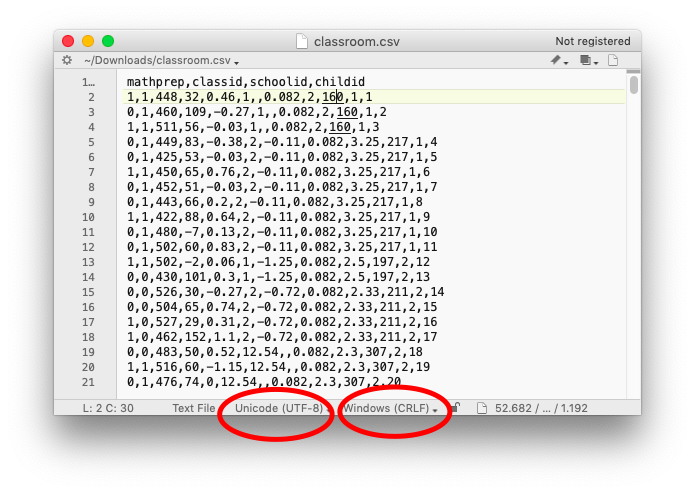
\includegraphics[width=0.9\linewidth]{figures/ch6_csv-in-editor}
\caption{A csv file opened in a text editor, illustrating that the columns are separated by commas, and showing the encoding and the line endings.}
\label{fig:csv-in-editor}
\end{figure}

As we will show in the practical code examples below, you can also force Python and R to use a specific encoding, which can come in handy if your data arrives in a legacy encoding.

Related to the different encodings a file can have, but less problematical, are different conventions of how a \emph{line ending} is denoted. Windows-based programs have been using a Carriage Return followed by a Line Feed (denoted as \texttt{\textbackslash r\textbackslash n}), very old versions of MacOS used a Carriage Return only (\texttt{\textbackslash r}), and newer versions of MacOS as well as Linux use a Line Feed only (\texttt{\textbackslash n}). In our field, the Linux (or Unix) style line endings have become most dominant, and Python 3 even automatically converts Windows style line endings to Unix style line endings when reading a file -- even on Windows itself.

A third difference is the use of so-called \emph{byte-order markers} (BOM). In essence, a BOM is an additional byte added to the beginning of a text file to indicate that it is a UTF-encoded file and to indicate in which order the bytes are to be read (the so-called endianness). While informative, this can cause trouble if your program does not expect that byte to be there. In that case, you might either want to remove it or explicitly specify the encoding as such (e.g., 'utf-8-bom' instead of 'utf-8' in the examples below).


In short, the most standard form in which you probably want to encode your data is in UTF-8 with Linux-style line endings without the use of a byte-order marker.


In the case of reading and writing csv files, we thus need to know the encoding, and potentially also the line ending conventions and the presence of a byte-order marker. However, there are also some additional variations that we need to consider. There is no single definition of how a csv file needs to look like, and there are multiple dialects that are widely used. They mainly differ in two aspects: the delimiter that is chosen, and the quoting an/or escaping of values.

First, even though csv stands for comma separated values, one could use other characters instead of a comma to separate the columns. In fact, because many countries use a comma instead of a dot to as a decimal separator (\$10.30 vs 10,30€), in these countries a semicolon (';') is used instead of a comma as  column delimiter. To avoid the possible confusion, others use a tab character (\texttt{\textbackslash t}) to seperate columns. Sometimes, these files are then called a tab-seperated file, and instead of .csv, they may have a file extension such as \ttt{.tsv}, \ttt{.tab}, or even \ttt{.txt}. However, this does not change the way how you can read them - but what you need to know is whether your columns are seperated by \texttt{,}, \texttt{;}, or \texttt{\textbackslash t}. 

Second, there may be different ways of how to deal with strings as values in a csv file. For instance, it may be that a specific value contains the same character that is also used as a delimiter. These cases are usually resolved by either putting all strings into quotes, putting only strings that contain such ambiguities in quotes, or by prepending the ambigous character with a specific escape character. Most likely, all of this is just handled automatically under the hood, but in case of problems, you might want to look into this and check out the documentation of the packages you are using on how to specify which strategy is to be used.

Let's get practical and try out reading and writing files into a data frame (\refex{readfiles}).

\pyrex[output=none, caption=Reading files into a dataframe]{chapter06/readfiles}

Of course, we can read more than just csv files. In the Python
example, you can use tabcompletion to get an overview of all file
formats Python supports: Type |pd.read| and then press the TAB key to
get a list of all supported files. For instance, you could to
|pd.read_excel('test.xlsx')|, |df3 = pd.read_stata('test.dta')|, or
|df4 = pd.read_json('test.json')| Similarily, for R, you can hit TAB
after typing |haven::| to get an overview over functions such as
|read_spss|.

\subsection{File handling beyond data frames}
Dataframes are a very useful data structure for organizing and analyzing data, and will come back in many examples in this book.
However, not all things that we might want to read from a file needs to go into a dataframe.
Imagine if we have a list of words that we later want to remove from some texts (so-called stopwords, see \refchap{protext}).
We could make a list (or vector) of such words directly in our code. 
But if we have more than a couple of such words, it is easier and more readable to keep them in an external file. We could create a file \texttt{stopwords.txt} in a text editor with one of such words per line:

\begin{lstlisting}
and
or
a
an
\end{lstlisting}

If you are too lazy to create this list yourself, you could also
download one from \url{http://cssbook.net/d/stopwords.txt} and save it
in the same directory as your Python or R script.

Then, you can read this file into a vector or list  (see \refex{readingstopwords}).

\pyrex[output=none, caption=Reading files without dataframes]{chapter06/stopwords}

\pyrex[output=none, caption={More examples for reading from and writing to files. Because dictionaries do not exist in R and handling non-rectangular data is more uncommon in R, we do not show an example for direct interaction with JSON files without involvement of a dataframe in the R example.}]{chapter06/extendedfilehandling}

\refex{extendedfilehandling} provides you with some more elaborate code examples that allows us to dig a bit deeper into the general way of handling files.

In the Python example,  we can open a file and assign a handle to it that allows us to refer to it (the name of the handle is arbitrary, let's just call it \texttt{f} here.
Then, we can use a for loop to iterate over all lines in the file and add it to a list

The \texttt{mode = 'r'} specifies that we want to read from the file. \texttt{mode = 'w'} would open the file for writing, create it if necessary, and immediately deletes all content that may have been in there if the file already existed (!).
Note that the \texttt{.strip()} is necessary to remove the line ending itself, and also possible whitespace at the beginning or end of a line.
If we want to save our stopwords, we can do this in a similar way: We first open the file (this time, for writing), and then use the file handle's methods to write to it.
We are not limited to plain text files, here. For instance, we can use the same approach to read json files into a python dict or to store a python dict into a json file.

We could also combine this with a for loop that goes over all files in a dictionary.
Imagine we have a folder full of positive movie reviews, and another one full of negative movie reviews that we want to use to train a machine learning classifier (see Section~\ref{sec:supervised}).
Let's further assume that all these reviews are saved as \texttt{.txt} files.
We can iterate over all of them, as shown in \refex{reviewdata}. If you want to read text files into a dataframe in R, the \pkg{readtext} package may be interesting for you.


\section{Data from online sources}
\label{sec:gathering}

Many data that are interesting to those analyzing communication are
nowadays gathered online.  In Chapter~\ref{chap:scraping}, you will
learn how to use APIs to retrieve data from web services, and how to
write your own web scraper to automatically download large quanties of
web pages and extract relevant information. For instance, you might
want to retrieve customer reviews from a website or articles from news
sites.

In this section, however, we will focus on how to re-use existing
datasets that others have made available online. For instance, the
open science movement has led to more and more datasets being shared
openly using repositories such as Dataverse, Figshare, or
others. Re-using existing data can be very good for several reasons:
First, to confirm (or not) the conclusions drawn by others; second, to
not waste resources by re-collecting very similar or even identical
data all over again; and third, because gathering a large,
high-quality dataset might just not be feasible with your means. This
is especially true when you need annotated (i.e., hand-coded) data for
supervised machine learning purposes (Chapter~\ref{chap:introsml}).

We can distinguish between two types of existing online datasets:
datasets that are inherently interesting, and so-called toy datasets.

Toy datasets may include made-up data, but often, these data are
real. However, they are not analyzed to gain scientific insights (any
more), as they may be too small, outdated, or already analyzed
all-over again. These provide a great way, though, to learn and
explore new techniques: After all, the results and the characteristics
of the data are already known. Hence, such toy datasets are often
even included in R and Python packages. Some of them are really
well-known in teaching (e.g., the iris dataset containing measurements
of some flowers; or the titanic dataset containing statistics on
survival rates of passengers on the Titanic; or the MPG dataset on car fuel consumption). Many of these are included
in packages like \pkg{scikit-learn}, \pkg{seaborn}, or \pkg{ggplot2}-- have a look at their documentation.

For instance, the 20 Newsgroups dataset contains $18,846$ posts from
newsgroups plus the groups where they were posted
(\refex{20newsgroups}). This can be an interesting resource for
exercising with natural language processing, unsupervised, and
supervised machine learning. Another interesting resource are
collections of political speeches, such as the state-of-the-union
speeches from the US, which are available in multiple packages
(\refex{sotudata}).
Other interesting datasets with large collections of textual data may
be the Financial News dataset compiled by \cite{Chen2017} or the
political news dataset compiled by \cite{Horne2018}.


\pyrex[output=py, input=both,caption={In Python, \pkg{scikit-learn} has a convenience function to automatically download the 20 newsgroup dataset and automatically clean it up. In R, you can download the raw version (there are multiple copies floating around on the internet) and perform the cleaning yourself.}]{chapter06/20newsgroups}

\pyrex[output=r, input=both, format=table, caption={A collection of US state-of-the-union speeches is available in multiple packages in various forms.}]{chapter06/sotudata}



There are also some more generic ressources that you may want to consider for finding
more datasets to play around with. On  \url{https://datasetsearch.research.google.com},
you can search for datasets of all kinds, both really interesting ones and toy datasets.
Another great research is \url{https://kaggle.com}, a site that hosts data
science competitions.






\setcounter{chapter}{8}
\chapter{Introduction to Statistical Modeling and Supervised Machine Learning}
\label{chap:introsml}
In this chapter, we introduce the basic concepts and ideas behind
machine learning.  We will outline how machine learning relate to
traditional statistical approaches that you already might now (and as
you will see, there is a lot of overlap), present different types of
models, and discuss how to validate them.

In a later chapter (Chapter~\ref{chap:text}), we will then
specifically apply the knoweldge you gained from this chapter to the
analysis of textual data, arguably one of the most interesting tasks
in the computational analysis of communication.

In this chapter, we mostly focus on \emph{supervised} machine learning
-- a form of machine learning, where we aim to predict a variable
that, for at least a part of our data, is known. To illustrate the
idea, imagine that you are interested in predicting the gender based
on Twitter biographies. You determine the gender for some of the
biographies yourself and hand these examples over to the computer. The
computer ``learns'' from your examples, and can then be used to
predict the gender for other twitter biographies for which you do not
know the gender.

In unsupervised machine learning, in contrast, you do not have such
examples. We have discussed some of such techniques in [ADD REFERENCE
  TO EXPLORATIVE DATA CHAPTER], in particular cluster analysis and
principal component analysis (PCA)/singular value decomposition (SVD).
Later, in chapter [ADD REFERENCE TO TOPIC MODELLING CHAPTER], we will
discuss topic models, an unsupervised method to extract so-called
topics from textual data.

Even though both approaches can be combined (for instance, one could
first reduce the amount of data using SVD, and then predict some
outcome), they can be seen as fundamentally different, also from a
theoretical and conceptual point of view.  Unsupervised machine
learning is a bottom-up approach and corresponds to an inductive
reasoning: you do not have a hypothesis of, for instance, which topics
are present in a corpus of text; you rather let the topics emerge from
the data.  Supervised machine learning, in contrast, is a top-down
approach and can be seen as more deductive: you define a priori which
topics to predict.

Both supervised and unsupervised approaches are widely used in the computational analysis of communication, and you will meet them across the book.
In this chapter, however, we will focus on supervised learning.

\section{Statistical modeling and prediction}
\label{sec:prediction}
Machine learning, many people joke, is nothing else than a fancy name
for statistics.  And, in fact, there is some truth to this: If you say
``logistic regression,'' this will sound familiar to both
statisticians and machine learning practitioners.  Hence, it does not
make much sense to distinguish between statistics on the one hand and
machine learning on the other hand.

Still, there are some differences between traditional statistical
approaches that you may have learned about in your statistics classes
and the machine learning approach, even if they use some of the same
mathematical tools. One may say that  the focus is a different
one, and the objective we want to achieve may differ.

Let us illustrate this with an example.
\texttt{mediause.csv}\footnote{You can download the file from
  \url{http://cssbook.nl/d/mediause.csv}} contains a few columns from
survey data on how many days per week respondents turn to different
media types (\emph{radio}, \emph{newspaper}, \emph{tv} and \emph{internet}) in order to follow the news\footnote{For a detailed
  description of the dataset, see \citet{Trilling2013phd}.}. It also
contains their \emph{age} (in years), their \emph{gender} (coded as female = 0, male = 1), and their \emph{education} (on a 5-point scale).

A straightforward question to ask is how far the
sociodemographic characteristics of the respondents explain their
media use.  Social scientists would typically approach this question
by running a regression analysis.  Such an analysis tells us how some
independent variables $x_1, x_2 \ldots x_n$ can explain $y$.  In an
ordinary least square regression (OLS), we would estimate $y=\beta_0 +
\beta_1 x_1 + \beta_2 x_2 + \ldots + \beta_n x_n$.

In a typical social-science paper, we would then interpret the coefficients
that we estimated, and say something like: When $x_1$ increases by one unit,
$y$ increases by $\beta_1$.
We sometimes call this ``the effect of $x_1$ on $y$'' (even though, of course,
it depends on the study design weather the relationship can really be interpreted
as a causal effect).
Additionally, we might look at the explained variance $R^2$, to assess how good the model fits our data. In \refex{ols} we use this regression approach to model the relationship of \emph{age} and \emph{gender} over the number of days per week a person reads a \emph{newspaper}. We fit the linear model using the \pkg{stats} function \fn{lm} in R and the \pkg{statsmodels} (module formula.api) function \fn{ols} in Python.

\pyrex[output=py, caption=Obtaining a model through estimating an OLS regression]{chapter09/ols}

Most traditional social-scientific analyses stop after reporting and
interpreting the coefficients of \emph{age} ($\beta = 0.0676$) and \emph{gender} ($\beta = -0.0896$), as well as the total explained variance (19\%) of such a model for our dependent variable \emph{newspaper}.
But we can go a step further. Given that we have already estimated our
regression equation, why not use it to do some \textit{prediction}?

We have just estimated that

$\textrm{newspaperreading} = -0.0896 + 0.0676 \cdot \textrm{age} + 0.1767 \cdot \textrm{gender}$

By just filling in the values for a 20 year old man, or a 40 year old
woman, we can easily calculate the expected number of days such a
person reads the newspaper per week, \emph{even if no such person
  exists in the original dataset}.

We learn that

$\hat{y}_{man20} = -0.0896 + 0.0676 \cdot 20 + 1 \cdot 0.1767 = 1.4391$

$\hat{y}_{woman40} = -0.0896 + 0.0676 \cdot 40 + 0 \cdot 0.1767 = 2.6144$

This was easy to do by hand, but of course, we could do this automatically for a large and essentially unlimited number of cases.
This could be as simple as shown in \refex{olspredict}.

\pyrex[output=py, caption=Using the OLS model we estimated before to predict the dependent variable for new data where the dependent variable is unknown.]{chapter09/olspredict}

In doing so, we shift our attention from the interpretation of coefficients to the prediction of the dependent variable for new, unknown cases. We do not
care about the actual values of the coefficents, we just need them for our prediction.
In fact, in many machine learning models, we will have so many of them that
we do not even bother to report them.

As you see, this implies that we proceed in two steps: First, we use some data
to estimate our model. Second, we use that model to make predictions.

We used an OLS regression for our first example, because it is very
straightforward to interpret and most of our readers will be familiar
with it.  However, a model can take the form of \emph{any} function,
as long as it takes some characteristics (or ``features'') of the
cases (in this case, people) as input and returns a prediction.

Using such a simple OLS regression approach for prediction, as we did in our example, can come with a couple of problems, though. One problem is that in some cases, such predictions do not make much sense. For instance, even though we know that the output should be something between 0 and 7 (as that is the number of days in a week), our model will happily predict that once a man reaches the age of 105 (rare, but not impossible), he will read a newspaper on 7.185 out of 7 days. Similarly, a one year old girl will even have a negative amount of newspaper reading. A second problem relates to the models' inherent assumptions. For instance, in our example it is quite an assumption to make that the relationships between these variables are linear – we will therefore discuss multiple models that do not make such assumptions later in this chapter. And, finally, in many cases, we are actually not interested in getting an accurate prediction of a continuous number (a \textit{regression} task), but rather in predicting a category. We may want to predict whether a tweet goes viral or not, whether a user comment is likely to contain offensive language or not, whether an article is more likely to be about politics, sports, economy, or lifestyle. In machine learning terms, these tasks are known as \textit{classification}.

In the next section, we will outline key terms and concepts in machine
learning. After that, we will discuss specific models that you
can use for different use applications.


\section{Concepts and Principles}
\label{sec:principles}

%\label{sec:supervised}
The goal of Supervised Machine Learning can be summarized in one sentence:
Estimate a model based on some data, and then use the model to predict the
expected outcome for some new cases, for which we do not know the outcome yet.
This is exactly what we have done in the introductory example in Section~\ref{sec:prediction}.

But when do we need it?

In short, in any scenario where the following two preconditions are fulfilled.
First, we have a large dataset (say, $100,000$
headlines) for which we want to predict to which class they belong to (say, whether
they are clickbait or not).
Second, for a random subset of the data (say, $2,000$ of the headlines), we already
know the class.
For example because we have manually coded (``annotated'') them.

Before we start using SML, though, we first need to have
a common terminology.
At the risk of oversimplifying matters, Table~\ref{tab:mllingo} provides a rough
guideline of how some typical machine learning terms translate to statistical
terms that you may be familiar with.

\begin{table}
\caption{Some common machine learning terms explained\label{tab:mllingo}}{
  \centering
\begin{tabularx}{\textwidth}{XX}
\toprule
machine learning lingo  & statistics lingo\\ \midrule
feature                 & independent variable  \\
label                   & dependent variable  \\
labeled dataset         & dataset with both independent and dependent variables\\
to train a model        & to estimate \\
classifier (classification)  & model to predict nominal outcomes \\
to annotate             & to (manually) code (content analysis) \\
\bottomrule
\end{tabularx}}{}
\end{table}

Let us explain them more in detail by walking through a typical SML workflow.

Before we start, we need to get a \emph{labeled dataset}.
It may be given to us, or we need to create it ourselves.
For instance, often we can draw a random sample of our data and use techniques
of manual content analysis \citep[e.g.,][]{riffe2019analyzing} to
\emph{annotate} (i.e., to manually code) the data.
You can download an example for this process (annotating the topic of news
articles) from \url{http://dx.doi.org/10.6084/m9.figshare.7314896.v1} \citep{Vermeer2018}.

It is hard to give a rule of thumb for how much labelled data you need.
It depends heavily on the type of data you have (if it is a \emph{binary} or a \emph{multi-class} classification problem), and on how evenly distributed (\emph{class balance}) they are (after all, having $10,000$ annotated headlines doesn't help you if $9,990$ are no clickbait and only $10$ are).
These reservations notwithstanding, it is fair to say that typical sizes in
our field are (very roughly) speaking often in the order of $1,000$ to $10,000$
when classifying longer texts \citep[see][]{Burscher2014},
even though researchers studying less rich data sometimes annotate larger
datasets \citep[e.g., $60,000$ social media messages in][]{vermeer2019seeing}.

Once we have established that this labelled dataset is available and
have ensured that it is of good quality, we randomly split it into two
datasets: a \emph{training dataset} and a \emph{test
  dataset}.\footnote{In Section~\ref{sec:validation}, we discuss more
  advanced approaches, such as splitting into training, validation,
  and test dataset, and cross-validation.}  We will use the first one
to train our model, and the second to test how good our model
performs. Common ratios range from 50:50 to 80:20; and especially if
the size of your labelled dataset is rather limited, you may want to
have a slightly larger training dataset at the expense of a slightly
smaller test dataset.

In \refex{preparedata}, we prepare the dataset we already used in
Section~\ref{sec:prediction} for classification by creating a
dichotomous variable (the label) and splitting it into a training and
a test dataset. We use |y_train| to denote the training labels and
|X_train| to denote the feature matrix of the training dataset;
|y_test| and |X_test| is the corresponding test dataset. We set a
so-called random-state seed to make sure that the random splitting
will be the same when re-running the code. We can easily split these datasets using the \pkg{rsample} function \fn{initial\_split} in R and the \pkg{sklearn} function \fn{train\_test\_split} in Python.

\pyrex[output=py, caption=Preparing a dataset for supervised machine learning]{chapter09/preparedata}

We now can \emph{train our classifier} (i.e., estimate our model using the
training dataset contained in the objects \texttt{X\_train} and \texttt{y\_train}). This can be as straightforward as estimating a
logistic regression equation (we will discuss different classifiers in
Section~\ref{sec:nb2dnn}).  It may be that we first need to create new
independent variables, so-called features, a step known as
\emph{feature engineering}, for example by transforming existing
variables, combining them, or by converting text to numerical word
frequencies.
\refex{nb} shows how easy it is to train a classifier using the Na\"ive Bayes algorithm with packages \pkg{caret}/\pkg{naivebayes} in R and \pkg{sklearn} in Python (this approach will be better explained in Subsection~\ref{subsec:naivebayes}).

\pyrex[output=none, caption=A simple Na\"ive Bayes classifier]{chapter09/nb}

But before we can actually use this classifier to do some useful work, we need to test how capable it actually is to predict the
correct labels, given a set of features. One might think that we could
just feed it the same input data (i.e., the same features) again and
see whether the predicted labels match the actual labels of the test
dataset.  In fact, we could do that.  But this test would not be
strict enough: After all, the classifier has been trained on exactly
these data, and therefore one would expect it to perform pretty well.
In particular, it may be that the classifier is very good in
predicting its own training data, but fails at predicting other data,
because it overgeneralizes some idiosyncrasy in the data, a phenomenon
known as overfitting (see Figure ~\ref{fig:overfit}).

\begin{figure} 
\centering
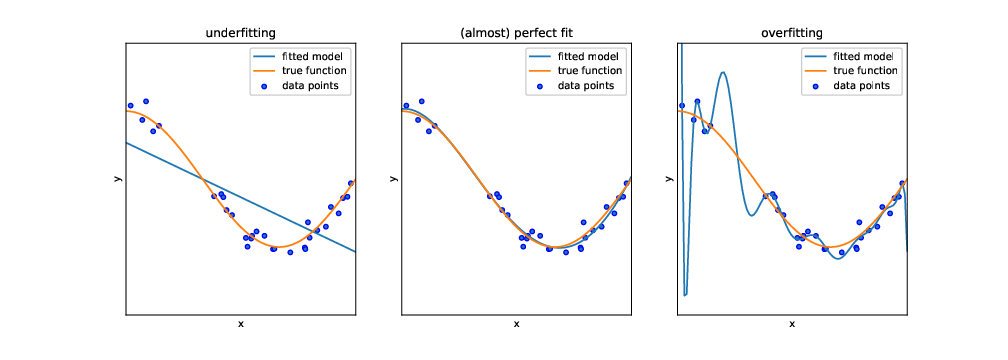
\includegraphics[width=\linewidth]{figures/ch09_overfitting}
\caption{Underfitting and overfitting. Example adapted from https://scikit-learn.org/stable/auto\_examples/model\_selection/plot\_underfitting\_overfitting.html}
\label{fig:overfit}
\end{figure}

Instead, we use the features of the \emph{test dataset} (stored in the objects  \texttt{X\_test} and \texttt{y\_test})  as input for
our classifier, and evaluate in how far the predicted labels match the
actual labels.  Remember: the classifier has at no point in time seen
the actual labels.  Therefore, we can in fact calculate how often the
prediction is right.\footnote{We assume here that the manual annotation
  is always right; an assumption that one may, of course,
  challenge. However, in the absence of any better proxy for reality,
  we assume that this manual annotation is the so-called \emph{gold
    standard} that reflects the \emph{ground truth} as closely as
  possible, and that it by definition cannot be outperformed. When creating the manual annotations, it is therefore important to safeguard their quality. In particular, one  should calculate and report some reliability measures, such as the \emph{intercoder reliability} which tests the degree of agreement between two or more annotators in order to check if our classes are well defined and the coders are doing their work correctly.}

\pyrex[output=py, caption=Calculating precision and recall]{chapter09/classificationreport}

As shown in \refex{classificationreport}, we can create a \emph{confusion matrix} (generated with \pkg{caret} function \fn{confusionMatrix} in R and \pkg{sklearn} function \fn{confusion\_matrix} in Python), and then estimate two measures: \emph{precision} and \emph{recall} (using base R calculations in R and \pkg{sklearn} function \fn{classification\_report} in Python). In a binary classification, the \emph{confusion matrix} is a useful table in which each column usually represents the number of cases in a predicted class, and each row the number of cases in the real or actual class. With this matrix (see \reffig{matrix}) we can then estimate the number of \emph{true positives} (TP) (correct prediction), \emph{false positives} (FP) (incorrect prediction), \emph{true negatives} (TN) (correct prediction) and \emph{false negatives} (FN) (incorrect prediction).


\begin{figure} 
\centering
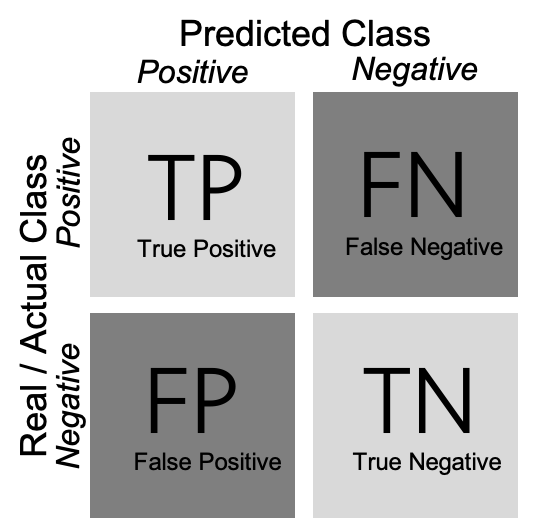
\includegraphics[width=\linewidth]{figures/ch09_matrix}
\caption{Visual representation of a confusion matrix}
\label{fig:matrix}
\end{figure}

For a better understanding of these concepts, imagine that we build a sentiment classifier, that predicts -- based on the
text of a movie review -- whether it is a positive review or a
negative review. Let us assume that the goal of training this classifier is to build an app that recommends the user only good movies. There are two things
that we want to achieve: We want to find as many positive films as possible (recall), but we also want that the selection we found
\emph{only} contains positive films (precision).

Precision is calculated as $\frac{TP}{TP+FP}$, where TP are true
positives and FP are false positives. For example, if our classifier
retrieves 200 articles that it classifies as positive films, but only
150 of them indeed are positive films, then the precision is
$\frac{150}{150+50} = \frac{150}{200} = 0.75$.

Recall is calculated as $\frac{TP}{TP+FN}$, where TP are true
positives and FN are false negatives. If we know that the classifier
from the previous paragraph missed 20 positive films, then the recall
is $\frac{150}{150+20} = \frac{150}{170}= 0.88$.

In other words: Recall measures how many of the cases we wanted to
find we actually found. Precision measures how much of what we have
found actually is correct.

Often, we have to make a trade-off between precision and recall. For
example, just retrieving \emph{every} film would give us a recall of
1.0 (after all, we didn't miss a single positive film). But on the
other hand, we retrieved all the negative films as well, so precision
will be extremely low. It can depend on the task at hand whether
precision or recall is more important. In
Section~\ref{sec:validation}, we discuss this tradeoff in detail, as well as other metrics such as \emph{accuracy}, \emph{f1-score} or the \emph{area under the curve} (AUC).


\section{From Na\"{i}ve Bayes to Deep Neural Networks}
\label{sec:nb2dnn}


\section{Validation and best practices}
\label{sec:validation}
\subsection{Finding a balance between precision and recall}
\label{sec:balance}

In the previous sections, we have learned how to fit different models:
Na\"ive Bayes, logistic regressions, support vector machines, and
random forests.  We have also had a first look at confusion matrices,
precision, and recall.

But how do we find the best model? ``Best'', here, should be read as
``best for our purposes'' -- some models may be bad, and some may be
good, but which one is really the best may depend on what matters most
for us: Do we care more about precision or about recall? Are all
classes equally important to us?  And of course, other factors, such
as explainability or computational costs may factor into our decision.
 
But in any event, we need to decide which metrics to focus on.  We can
then either manually inspect them and look, for instance, which model
has the highest \emph{accuracy}, or the best balance of precision and recall,
or a recall higher than some threshold you are willing to accept.

If we build a classifier to distinguish spam messages from legitimate
messages, we could ask the following questions:
\begin{description}
\item[Precision] Which percentage of what our classifier predicts to be
  spam really is spam?
\item[Recall]{What percentage of all spam messages has our classifier
  found?}
\item[Accuracy]{In which percentage of all cases was our classifier
  right?}
\end{description}

We furthermore have:
\begin{description}
\item[F1-score]{The harmonic mean of precision and recall: $F_1 = 2
  \cdot \frac{precison \cdot recall}{precison + recall}$}
\item[AUC]{The AUC (Area under Curve) is the area under the curve that
  one gets when plotting the True Positive Rate (TPR) against the
  False Positive Rate (FPR) at various threshold settings. A perfect
  model will receive a value of 1.0, while random guessing between two
  equally probable classes will result in a value of 0.5}
\item[Micro- and macroaverage]{Especially when we have more than two
  classes, we can calculate the average of measures such as precision,
  recall, or f1-score. We can do so based on the separately calculated
  measures (macro), or based on the underlying values (TP, FP, etc.)
  (micro), which has different implications in the interpretation --
  especially if the classes have very different sizes.}
\end{description}


So, which one to choose?  If we really do not want to be annoyed by
any spam in our inbox, we need a high recall (we want to find all spam
messages). If, instead, we want to be sure that we do not
accidentally throw away legitimate messages, we need a high
precision (we want to be sure that all spam really is spam).

Maybe you say: well, I want both!  You could look at the accuracy, a
very straightforward to interpret measure. However, if you get many
more legitimate messages than spam (or the other way round), this
measure can be misleading: after all, even if your classifier finds
almost none of the spam messages (it has a recall close to zero), you
still get a very high accuracy, simply because there are so many
legitimate messages. In other words, the accuracy is not a good measure when working with highly unbalanced classes.
Often, it is therefore a better idea to look at the harmonic mean of
precision and recall, the F1-score, if you want to find a model that
gives you a good compromise between precision and recall.


In fact, we can even fine-tune our models in such a way that they are
geared towards either a better precision or a better recall.
As an example, let us take a logistic regression model. It predicts a
class label (such as ``spam'' versus ``legitimate''), but it can also
return the assigned probabilities. For a specific message, we can thus
say that we estimate its probability of being spam as, say, .65.
Unless we specify otherwise, everything above .5 will then be judged
to be spam, everything below as legitimate. But we could specify a
different cutoff point: we could, for instance, decide to classify
only everything above .7 as spam. This would give us a more
conservative spam filter, with probably a higher precision at the
expense of a lower recall.

\begin{figure} 
\centering
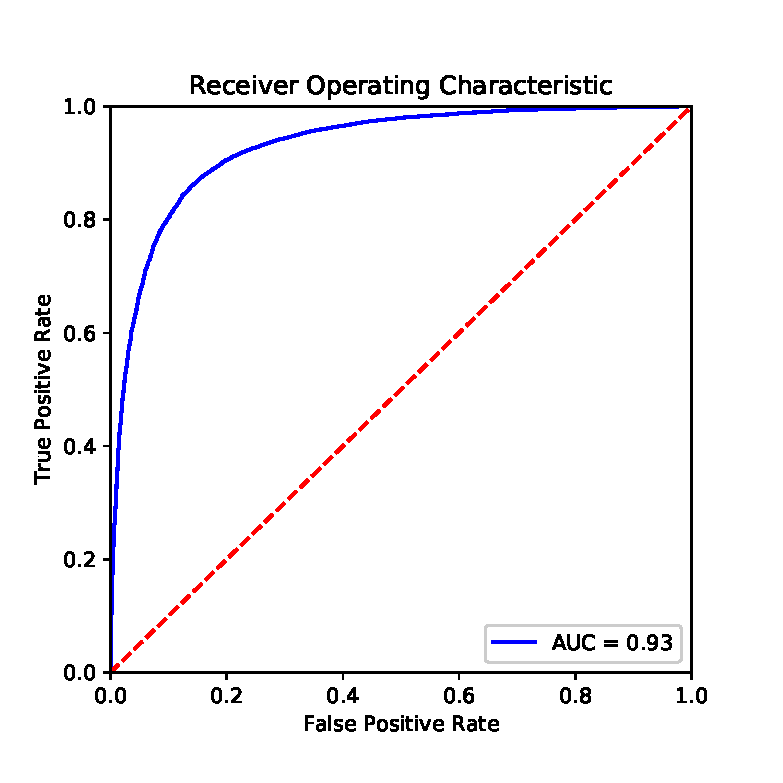
\includegraphics[width=0.4\linewidth]{figures/ch09_roccurve}
\caption{A ROC curve.}
\label{fig:roccurve}
\end{figure}

We can visualize this with a so-called ROC (reveicer operator
chraracteristic), a plot in which (Figure~\ref{fig:roccurve}) we plot
true positives against false positives at different thresholds.  A
good model extends until close to the upper left corner, and hence has
a large area under the curve (AUC).  If we choose a threshold at the
left end of the curve, we get few false positives (good!), but also
few true positives (bad!), if we go too far to the right, we get
the other extreme. So, how can we find the best spot?

One approach would be to print a table with three columns: the false
positive rate, the true positive rate, and the threshold value. You
then decide which FPR-TPR combination is most appealing to you, and
use the corresponding threshold value.

The second approach (also knwon as Yoden's J) is to find the threshold
value with the maximum distance between TPR and FPR, and use that one.

\pyrex[input=py, output=py,caption={Choosing a differnet cutoff point for predictions with logistic regression. In this case, we make a tradeoff and maximize the difference between false positive rate and true positive rate to improve the precision for the the second categegory by .12 at the expense of reducing the precision for the first category by .8.}]{chapter09/cutoffpoint}


\subsection{Train, validate, test}
\label{sec:train}

By now, we have established which measures we can use to decide which
model to use. For all of them, we have assumed that we split our
labeled dataset into two: a training dataset and a test dataset. The
logic behind it was simple: If we would calculate precision and recall
on the training data itself, our assessment would be too optimistic --
after all, our models have been trained on exactly these data, so
predicting the label isn't too hard. Assessing the models on a different
dataset, the test dataset, instead, gives us an assessment of how
precision and recall look like if haven't seen the labels earlier --
which is exactly what we want to know.

Unfortunately, if we calculate precision and recall (or any other
metric) for multiple models on the same test dataset, and use these
results to determine which metric to use, we can run into a problem:
We may avoid overfitting of our model on the training data, we may now
overfit it on the test data! After all, we could tweak our models as
long until they fit our test data perfectly, even if this makes the
predictions for other cases worse.

One way to avoid this is to split the original data into three
datasets instead of two: a training dataset, a validation dataset, and
a test dataset.  We train multiple model configurations on the
training dataset and calculate the metrics of interest for all of them
on the validation dataset.  Once we have decided on a final model, we
calculate its performance (once) on the test dataset, to get an
unbiased estimate of its performance.



\subsection{Cross-validation and grid search}
\label{sec:crossvalidation}
In an ideal world, we would have a huge labelled dataset and do not
need to worry about the decreasing size of our training dataset as we
set aside our validation and test datasets.

Unfortunately, our labelled datasets in the real world have a limited
size, and setting aside too many cases can be problematic. Especially
if you are already on a tight budget, setting aside not only a test
dataset, but also a validation dataset of meaningful size may lead to
critically small training datasets. While we have addressed the
problem of overfitting, this could lead to underfitting: We may have
removed the only examples of some specific feature combination, for
instance.

A common approach to address this issue is $k$-fold
cross-validation. To do so, we split our data into $k$ partitions,
so-called folds. We then estimate our model $k$ times, and each time
leave \emph{one} of the folds aside for validation. Hence, every fold
is exactly one time the validation dataset, and exactly $k-1$ times
part of the training data. We then simply average the results of our
$k$ values for the evaluation metric we are interested in.

If our classifier generalizes well, we would expect that our metric of
interest (e.g., the accuracy, or the f1-score, \ldots) is very similar
in all folds. ~\refex{crossval} performs a cross-validation based on
the logistic regression classifier we build above. We see that the
standard deviation is really low, indicating that there are almost no
changes between the runs, which is great.

Running the same cross-validation on our random forest, instead, would
produce not only worse (lower) means, but also worse (higher) standard
deviations, even though also here, there are no dramatic changes
between the runs.

\pyrex[input=both, output=both,caption=Crossvalidation]{chapter09/crossval}

Very often, cross-validation is used when we want to compare many
different model specifications, for example to find optimal
hyperparameters.
Hyperparameters are parameters of the model that are not estimated
from the data. These depend on the model, but could for example be the
estimation method to use, the number of times a bootstrap should be
repeated, etc. A very good example are the hyperparameters of support
vector machines (see above): It is hard to know how soft our margins
should be (the $C$), and we may also be unsure about the right kernel
(\refex{gridsearch2}), or in the case of a polinomial kernel, how many
degrees we want to consider.

Using the help function (e.g., \fn{RandomForestClassifier?} in Python),
you can look up
which hyperparameters you can specify. For a random forest classifier,
for instance, this includes the number of estimators in the model, the
criterion, and whether or not to use
bootstrapping. \refex{gridsearch}, \ref{ex:gridsearch2}, and
\ref{ex:gridsearch3} illustrate how you can automatically assess which
values you should choose.

\pyrex[input=py, output=py,caption=A simple gridsearch in Python]{chapter09/gridsearch}

\pyrex[input=py,output=py,caption=A gridsearch in Python using multiple CPUs]{chapter09/gridsearch2}

\pyrex[input=r,output=r,caption={A gridsearch in R. Note that in R, not all parameters are ``tunable'' using standard \pkg{caret}. Therefore, an exact replication of the grid searches in \refex{gridsearch} and \refex{gridsearch2} would requires either manual comparisons or writing a so-called caret extension.}]{chapter09/gridsearch3} 

\begin{feature}
    Supervised machine learning is one of the areas where you really
    see differences between Python and R. While in Python, virtually
    all you need is available via \pkg{scikit-learn}, in R, we often
    need to combine \pkg{caret} with various libraries providing the
    actual models. In contrast, all components we need for machine
    learning in Python are developed within one package, which leads
    to less friction. This is what you see in the gridsearch examples
    in this section. In scikit-learn, \emph{any} hyperparameter can be
    part of the grid, but no hyperparameter has to be.  Note that in
    R, in contrast, you cannot (at least, not easily) put any
    parameter of the model in the grid. Instead, you can look up the
    ``tunable parameters'' which \emph{must} be present part of the
    grid in the caret documentation. This means that an exact
    replication of the grid searches in \refex{gridsearch} and
    \refex{gridsearch2} is not natively supported using \pkg{caret}
    and requires either manual testing or writing a so-called caret
    extension.

    While in the end, you can find a supervised machine learning
    solution for all your use cases in R as well, if supervised
    machine learning is at the core of your project, it may save you a
    lot of cursing to do this in Python.
\end{feature}





\backmatter
% bibliography, glossary and index would go here.

\begin{small}
\printbibliography
\end{small}


\end{document}
